\section{Gradient-Based Prompt Optimization} \label{sec:gradient_methods}
As mentioned in~\cref{sec:manual_prompts}, \perez achieve high attack success rates when carrying out a manual prompt injection attack against early GPT-3 LLMs in late 2022.
However, the effectiveness of early approaches, like the one proposed by Perez and Ribeiro, decreases over time.
This becomes evident, for example, when \hui re-evaluate the attack approach of \perez on more modern LLMs in late 2024.
They find that the attack prompts of \perez are unable to recover any part of a model's system prompt in the majority of the attacks~\cite{hui_pleak_2024}.\\

The ineffectiveness of older prompt injection attacks on modern models is likely due to adjusted fine-tuning.
Attack prompts from existing prompt injection attacks can be taken into account during the fine-tuning of new LLMs, which reduces the effectiveness of the attacks.
\deng prove that this works by fine-tuning models on their own attack prompts, which significantly reduces the effectiveness of the attacks~\cite{deng_attack_2023}.
Nevertheless, using existing prompt injection attacks to fine-tune new models does not make models fundamentally robust against attacks, which we further discuss in~\cref{sec:current_defenses}.
However, it does drive the innovation of new and adapted attack approaches, such as gradient-based attack prompt optimization.
In the following, we give an overview of these more recent approaches by the example of attack frameworks proposed by \hui and \shi and compare them to the attack approaches discussed in~\cref{sec:manual_prompts} and~\cref{sec:automated_prompts}.

\subsection{Loss Minimization Approach} \label{sec:loss_minimization}
The approaches of both \hui and \shi follow the same basic principle to create attack prompts for prompt injection attacks.
They define the attack prompt generation as an optimization problem, using a loss function $\mathcal{L}$ to quantify the deviation of the attacked model's actual response from the response targeted by the attack~\cite{hui_pleak_2024, shi_optimization-based_2024}.
For example, \shi use the negative log-likelihood of the embedding vectors $\textbf{r}_i$ that form the model's response to define the loss of an attack response.
When the model is given the adversarial prompt $\tilde{\textbf{p}}$, which was built with the injected instructions $\textbf{s}^e$, the model response aimed for by the attack can be expressed as a series of embedding vectors $\tilde{\textbf{r}^*} = \textbf{r}_1^*, \textbf{r}_2^*, ... \textbf{r}_{n_r}^*$.
Meanwhile the actual response $\tilde{\textbf{r}}$, which might differ from the intended response $\tilde{\textbf{r}*}$, can be equivalently expressed as $\tilde{\textbf{r}} = \textbf{r}_1, \textbf{r}_2, ... \textbf{r}_n$.
The loss of the proposed attack prompt $\tilde{\textbf{p}}$ can then be expressed as:
\begin{equation}
    \mathcal{L}(\tilde{\textbf{p}}) = -log \prod_{i=1}^{n_r} \text{Pr}(\textbf{r}_i^*|\tilde{\textbf{p}}, \textbf{r}_1, \textbf{r}_2, ..., \textbf{r}_{i-1})~\cite{hui_pleak_2024}
    \label{eq:optimization_loss}
\end{equation}
In other words, the loss is based on the probability that the model produces the attacker's desired output $\tilde{\textbf{r}^*}$ when injected with the malicious instructions $\tilde{\textbf{p}}$.
The objective of the attack prompt construction is then to find optimal attack prompts that minimize the loss:
\begin{equation}
    \underset{\tilde{\textbf{p}}}{\operatorname{argmin}} \; \mathcal{L}(\tilde{\textbf{p}})
\end{equation}
and therefore maximize the probability that the model's response is the desired output $\tilde{\textbf{r}^*}$~\cite{hui_pleak_2024, shi_optimization-based_2024}.\\

To iteratively find a solution to the optimization problem, \hui and \shi use gradient-based approaches~\cite{hui_pleak_2024, shi_optimization-based_2024}.
This is done in a three-step process.
In the first step, the responses of the model for a proposed attack prompt dataset are obtained by inputting the injected prompts into the model and collecting the corresponding output.
In the second step, the loss of the model's responses is calculated according to~\cref{eq:optimization_loss} while considering the attacker's desired responses for the corresponding attack.
In the third step, the attack prompts are updated to minimize the calculated loss by approximating the loss of updated attack prompts.
These three steps are carried out iteratively either for a certain number of iterations or until the algorithm converges.
The resulting attack prompt dataset then minimizes the defined loss and therefore maximizes the desired model response in prompt injection attacks on systems using that model.
The full iterative algorithm is conceptually depicted in~\cref{fig:optimization_alg}.\\

\begin{figure}[htb]
    \centering
    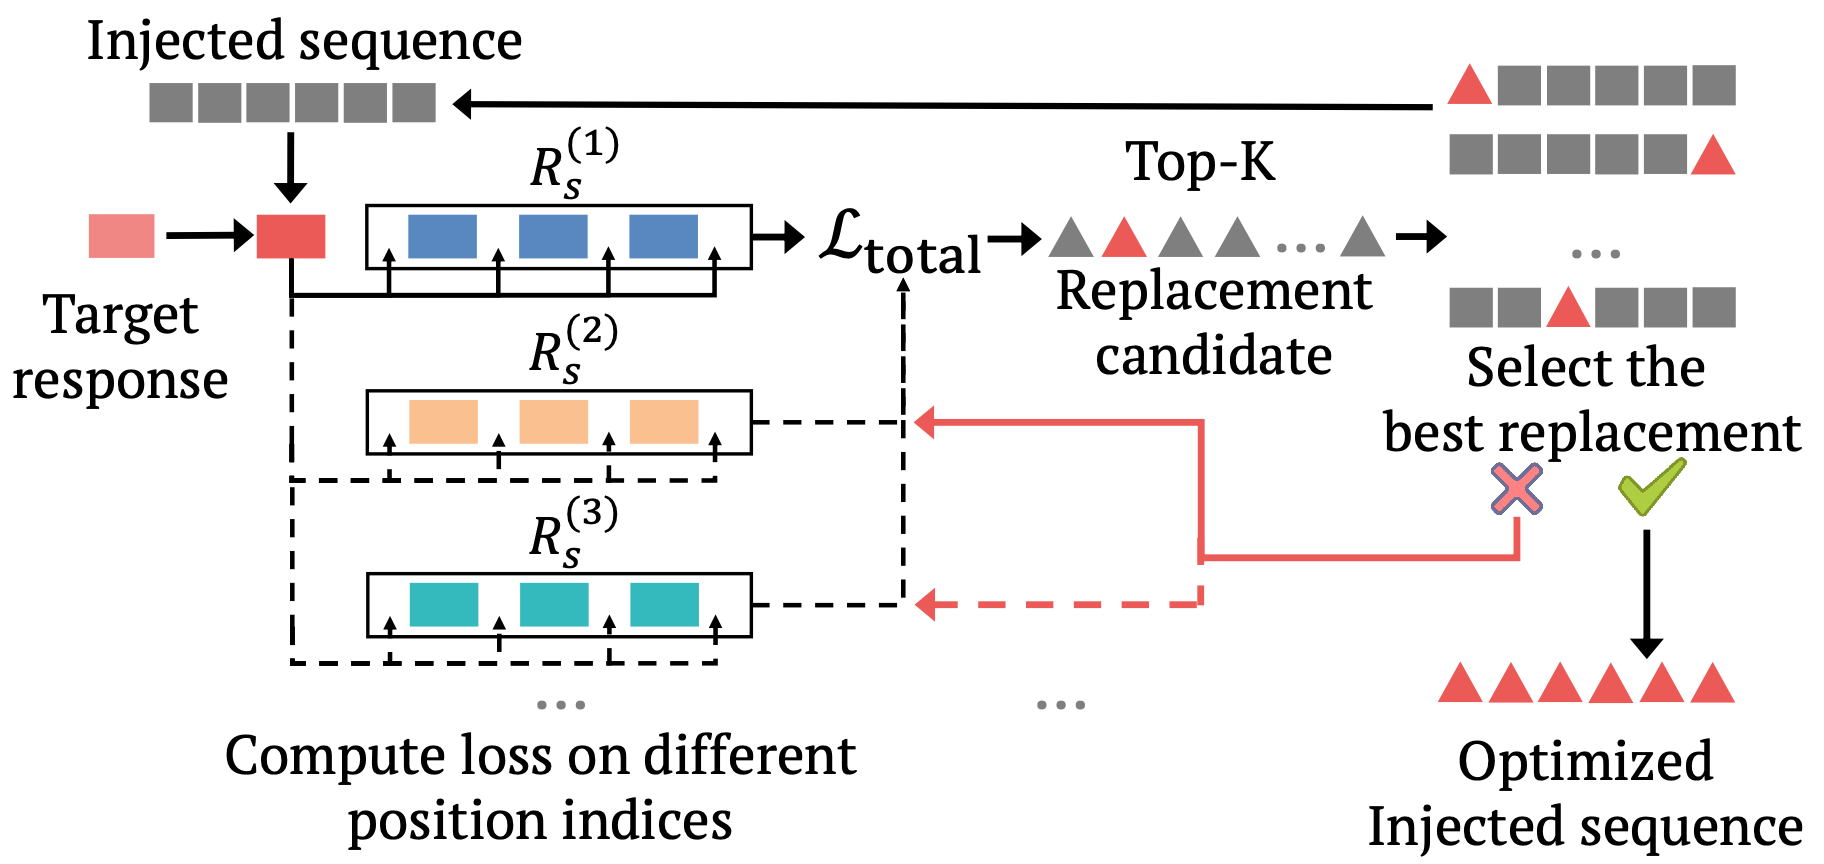
\includegraphics[width=\linewidth]{images/prompt_optimization.png}
    \caption{Iterative optimization of tokens in attack prompts based on a loss function~\cite{shi_optimization-based_2024}.}
    \Description[<>]{<>}
    \label{fig:optimization_alg}
\end{figure}

The main difficulty of this loss-based optimization approach is the discrete nature of the optimization problem.
In continuous gradient-descent approaches, the gradient of the loss is used to update the optimized parameter directly, typically by subtracting the gradient from the current iteration's input~\cite{russell_artificial_2021}.
However, not only the model's response $\tilde{\textbf{r}}$, but also the compromised prompt $\tilde{\textbf{p}} = \textbf{p}_1, \textbf{p}_2, ..., \textbf{p}_{n_p}$ are series of embedding vectors.
Therefore, updates to an attack prompt can only be made discretely by exchanging an embedding vector $\textbf{p}_i$ with an alternative embedding vector $\textbf{p}_i'$.
This means that no continuous updates can be made to the attack prompt.\\

Both \hui and \shi solve this problem by estimating the impact of changing individual embedding vectors in the attack prompt~\cite{hui_pleak_2024, shi_optimization-based_2024}.
If an updated attack prompt $\tilde{\textbf{p}}' = \textbf{p}_1, ..., \textbf{p}_i', ..., \textbf{p}_{n_p}$ is created by exchanging the embedding vector $\textbf{p}_i$ in $\tilde{\textbf{p}}$ with $\textbf{p}_i'$, the loss of the updated prompt can be expressed with~\cref{eq:optimization_loss} as $\mathcal{L}(\tilde{\textbf{p}}')$.
The loss of this updated attack prompt can then be approximated with a first-order Taylor expansion as:
\begin{equation}
    \mathcal{L}(\tilde{\textbf{p}}') \approx \textbf{p}_i' \;\ \nabla_{p_i} \mathcal{L}(\tilde{\textbf{p}})~\cite{hui_pleak_2024},
    \label{eq:loss_approx}
\end{equation}
where $\nabla_{p_i}$ denotes the gradient with respect to the $i$th embedding vector in $\tilde{\textbf{p}}$.
Notably, the approximation does not contain $\mathcal{L}(\tilde{\textbf{p}}')$, only $\mathcal{L}(\tilde{\textbf{p}})$.
This means that to evaluate the impact of a discrete update to the attack prompt, the updated prompt does not have to be fed through the model.
Therefore, the approximation allows for finding an optimal new embedding vector for each position $i$ in the attack prompt by searching through the set of discrete embedding vectors~\cite{hui_pleak_2024, shi_optimization-based_2024}.\\

Due to the presented approximation, it is not guaranteed that the update to the attack prompt that minimizes the approximated loss in~\cref{eq:loss_approx} also minimizes the true loss in~\cref{eq:optimization_loss}.
\hui and \shi mitigate this effect in a similar way.
They both find the $k$ best embedding vector updates for each position $i$ in the attack vector according to the approximated loss in~\cref{eq:loss_approx}~\cite{hui_pleak_2024, shi_optimization-based_2024}.
\hui then compute the true loss for each of the $k$ possible updates and find the optimal update amongst the $k$ pre-computed options~\cite{hui_pleak_2024}.
\shi use a greedy search with random sampling on the $k$ candidate updates instead~\cite{shi_optimization-based_2024}.

\subsection{Shadow Models}
While the loss-defined optimization approach presented in~\cref{sec:loss_minimization} allows for strategically choosing optimal updates to the attack prompts based on the attacked model's response, it does not conform to the threat model introduced in~\cref{sec:threat_model}.
Since computing the gradient in~\cref{eq:loss_approx} requires access to the LLM's internal weights and calculations, it is not possible to perform this optimization when only black-box access to the attacked model is assumed.\\

The naive solution to this is to change the threat model to assume white-box model access instead of black-box access.
However, this is not a realistic threat model for applications that use proprietary and closed-source LLMs.
Considering the fact that for many of the most capable and widely used LLMs like GPT-5~\cite{openai_introducing_2026}, Gemini 3~\cite{google_new_2025}, and Claude 4.5~\cite{anthropic_claude_nodate}, the internal weights are not available, this assumption would render gradient-based prompt injection attacks ineffective in many scenarios.
Both \hui and \shi opt for threat models that preserve the black-box access to the attacked application by using shadow models~\cite{hui_pleak_2024, shi_optimization-based_2024}.\\

Shadow models are used in the attack prompt optimization as a stand-in for the attacked model in the target application.
While the attacker only has black-box access to the LLM used in the attacked application, white-box access can be assumed for the shadow model~\cite{hui_pleak_2024, shi_optimization-based_2024}.
Several powerful LLMs are available under open-weight licenses, which can be used as shadow models.
\hui and \shi use, amongst others, models from the Llama~\cite{meta-llama-3-8b-instruct_2024} and Mistral~\cite{mistral_mistral-7b-instruct-v02_2023} families, as well as GPT-J~\cite{wang_eleutheraigpt-j-6b_2023}. 
Therefore, this hybrid threat model of white-box access to the shadow model and black-box access to the target model can be considered to be as strong as the threat model described in~\cref{sec:threat_model}.
During the attack prompt optimization, the shadow model is used together with a shadow dataset consisting of system and user prompts that are assumed to be similar to the ones encountered in an attack on the actual application~\cite{hui_pleak_2024, shi_optimization-based_2024}.
Whether actual data from the system can be collected by the attacker or whether assumptions have to be made to construct the shadow dataset depends on the additional attacker capabilities described in~\cref{sec:threat_model}.\\

Whether prompt injection attacks using shadow models are effective against the targeted application mainly depends on the transferability of the attack from the shadow model to the LLM used in the application.
Both \hui and \shi find that attacks trained on a shadow model that differs from the model used by the targeted application transfer with high effectiveness~\cite{hui_pleak_2024, shi_optimization-based_2024}.
While attack prompt effectiveness does decrease in some cases, especially when transferring an attack from a smaller shadow model to a larger target model, the attacks remain successful in most cases~\cite{hui_pleak_2024, shi_optimization-based_2024}.
Considering that an attacker might know which model is used by the targeted application, a suitable shadow model with proven high transferability and similar size can be chosen as the shadow model.
\hui also prove that attacks can remain highly effective even when the shadow dataset used in the attack prompt optimization significantly differs from data found in the target application~\cite{hui_pleak_2024}.

\subsection{Comparison to LLM-based Rephrasing}
The main advantage of the newer gradient-based approaches over the older approaches presented in~\cref{sec:manual_prompts} and~\cref{sec:automated_prompts} is their higher attack effectiveness on modern LLMs.
\hui find that in a prompt leaking scenario, their approach can recover an exact system prompt in up to $68\%$ of the attacks on modern LLMs, including \texttt{LLaMA-2-7B}~\cite{hui_pleak_2024}.
Compared to that, the attacks developed by \perez only recover the exact system prompt in $2\%$ of the attacks~\cite{hui_pleak_2024}.
Similarly, \shi achieve an average attack success rate of $97\%$ on the \texttt{Llama-3-8B-Instruct} model~\cite{shi_optimization-based_2024}.
Both \hui and \shi conclude that their newer gradient-based approaches are significantly more effective than previous prompt injection approaches on modern LLMs~\cite{hui_pleak_2024, shi_optimization-based_2024}.\\

The superior attack effectiveness of gradient-based methods can be attributed to their more direct optimization approach.
Manual or automated rephrasing approaches like the ones by \perez and \deng adjust attack prompts on a word level and base the updates made to attack prompts on general prompting rules and guidelines.
In contrast to that, gradient-based approaches like those by \hui and \shi adjust attack prompts on a token level and select attack prompt adjustments based directly on the attacked model's responses.
It can therefore be concluded that gradient-based methods are conceptually better suited to create attack prompts optimized for prompt injection attacks.
The better optimization does, however, come at the cost of the need for training data and a more complex attack prompt creation process.\\

Another advantage of gradient-based methods over rephrasing methods is that they are less dependent on the initial attack prompts used as a starting point for the optimization process.
\hui even find that an initialization with random embedding vectors is the best-performing initialization for their approach~\cite{hui_pleak_2024}.
Since the replacement of tokens in the attack prompt is chosen by searching through the token alphabet and not via in-context learning generation, gradient-based approaches are more likely to find optimized attack prompts that significantly differ from the initial prompts.
On the other hand, gradient-based approaches are dependent on a good transferability of the attack prompts from the shadow model they were optimized on to the model in the attacked application.
Since rephrasing-based approaches work without a shadow model, they tune the attack prompts directly on the attacked LLM.\\

The adjustment of gradient-based attacks to different attack goals is done by changing the loss function used for the optimization.
This not only allows for different attack goals but also enables additional specialization.
For example, \shi use three loss terms balanced by hyperparameters~\cite{shi_optimization-based_2024}.
One loss term aims at increasing the likelihood that the attack produces the desired response, similar to the loss defined in~\cref{eq:optimization_loss}.
The other two terms are introduced to make the attack robust against variations that are encountered in the attack scenario considered by \shi and to lower the attack prompt's perplexity to evade attack detection.
Introducing additional loss objectives and balancing the relative importance of loss terms allows for simple but effective specialization and adaption of gradient-based prompt injection attacks.

\subsection{Realistic Attack Scenarios} \label{sec:realistic_scenarios}
Another novelty of the prompt injection attacks proposed by \hui and \shi in comparison to older attacks like the ones by \perez and \deng is that they consider more realistic attack scenarios.
\hui do not only evaluate their attacks on offline applications but also test the effectiveness of their attack against real-world LLM applications on the Poe platform~\cite{hui_pleak_2024}.
For a prompt leaking attack against offline applications, they find an average success rate for recovering the exact system prompt is $82.3\%$.
While the average exact match on real-world applications is lower at $68.0\%$, it proves that their attack is suitable not only for attacks on experimental setups~\cite{hui_pleak_2024}.
\shi motivate their attack against LLM-as-a-judge applications with possible real-world targets like search result ranking, LLM tool selection frameworks, and reinforcement learning from AI feedback approaches~\cite{shi_optimization-based_2024}.
All of these areas are already using or will likely adopt LLM-as-a-judge-based evaluation and ranking and are therefore an attractive target for prompt injection attacks similar to the one proposed by \shi
In case studies to evaluate the efficacy of their attack against real-world applications in all three areas, \shi find that their attack is effective in all of them~\cite{shi_optimization-based_2024}.\\

Besides the more realistic attack targets, both \hui and \shi also consider the possibility of defenses against prompt injection attacks in their proposed attacks.
\hui use so called adversarial transformations to make their prompt leaking attack robust against output filters in the attacked applications.
In such a defense, the application searches for exact or partial matches of the system prompt in the LLM's output~\cite{hui_pleak_2024}.
\hui adjust their attack prompts to perform reversible transformations like prefixes to every sentence in order to evade possible output filters and then reverse the transformations on the attacker end~\cite{hui_pleak_2024}.
\shi use an additional balanced loss term to make a low perplexity of the attack prompts one of the optimization targets.
This approach can help to evade defenses based on the fact that optimized adversarial prompts often have higher perplexity than typical user prompts~\cite{shi_optimization-based_2024}.